\documentclass[a4paper]{jpconf}
\usepackage{graphicx}
\begin{document}
\title{An atmospheric electric field monitoring station for studying variations of cosmic ray flux at ground level during thunderstorms}

\author{P. Salgado-Meza, L. Florez-Villegas}

\address{Escuela de Ingenier\'ia El\'ectrica, Electr\'onica y de Telecomunicaciones, Universidad Industrial de Santander, Bucaramanga-Colombia}

\author{J. Pe\~na-Rodr\'iguez, L. A. N\'u\~nez}

\address{Escuela de F\'{\i}sica, Universidad Industrial de Santander, Bucaramanga-Colombia}

\ead{jesus.pena@correo.uis.edu.co}

\begin{abstract}
In this work, we expose the preliminary results of the implementation of a weather station for monitoring the atmospheric electric field and lightning during thunderstorm episodes for studying its effect on the secondary particle flux at ground level in cosmic ray observatories. The atmospheric electric field during thunderstorms can increase above hundreds of kV/m causing an acceleration in charged particles composing secondaries cosmic rays. Such acceleration causes avalanches processes in the atmosphere enhancing or reducing the particle flux at ground level depending on the strength and polarity of the electric field. 

\end{abstract}

\section{Introduction}
Cosmic rays (CRs) are high energy particles reaching the Earth after crossing the interstellar space. Most CRs originate outside the solar system and only low-energy ($<$ 10 GeV) particles are of solar origin. When such particles enter the terrestrial atmosphere, they interact with the atoms generating Extended Air Showers (EAS) of secondary particles \cite{Spurio2015}.

Secondaries are mainly charged particles like electrons and positrons which can be affected by the atmospheric electric field experimenting an acceleration \cite{marshall2005observed} which causes Relativistic Runaway Electron Avalanches (RREA) \cite{dwyer2011low} increasing the secondary flux at ground level. The atmospheric electric field can rise up to hundreds of 100 kV/m during thunderstorm episodes. The minimum electric field for triggering an RREA is roughly 286 kV/m \cite{Skeltved2017, colalillo2019}.

Wang et al. \cite{wang2012effect} and Alexeenko et al. \cite{alexeenko2002transient} concluded that the number of detected muons at ground level is modulated due to the strength of the atmospheric electric field. Additionally, Bartoli et al. \cite{bartoli2018observation} observed a decrease in the electron flux recorded by ARGO-YBJ during thunderstorm events, while Huang et al. \cite{zhao2019effects} found that the variation of electrons and gamma photons depend on the electric field polarization.

During negative electric fields, negative charge particles are accelerated towards the ground enhancing the particle counting at the detector level. On the other hand, in the presence of a positive electric field, the counting ratio at ground level decreases \cite{dorman2013cosmic}. These observations give an explanation of the electron/positron flux variation which has been observed by CRs observatories during thunderstorms \cite{Marteau-etal2012}.
Strong electromagnetic pulses emitted by lightning also generate unusual radiation events called ELVES (Emission of Light and Very Low-Frequency perturbations due to Electromagnetic Pulse Sources) at the ionosphere. Such phenomena and its correlation with lightning discharges have been studying at the Pierre Auger Observatory \cite{Mussa2019}. 

The main drawback in the understanding of the atmospheric electric field and its influence on the particle flux is the lack of electric field monitoring networks inside CR observatories for data cross-checking between the secondary counting rate and the electric field transitories.

For that reason, we present the development of a modular monitoring station capable to measure slow ($<$ 100 Hz) and fast ($<$ 500 KHz) changes in the atmospheric electric field during thunderstorm episodes. The station allows us to create a temporally synchronized network for finding correlations between secondary flux and electric field variations, as well as, it is able to estimate the localization of lightning strike points. Here, we show only the results of the slow component monitoring device. 

\section{Electric field mill}
E-filed mills are widely used to measure slowly-varying electric fields in a timescale of seconds associated with cloud charging processes. In this sensor, the steady electric field is shielded and unshielded by a moving grounded shutter placed over a sensing electrode. The charge induced on the sensitive electrode flows to the ground when the shutter screens the external electric field and flows back to the sensing electrode when it is uncovered. Then, the resulting sinusoidal current is proportional to the electric field magnitude \cite{Rakov2016}.  

The implemented E-field sensor is composed of three Bakelite plates (shutter, sensing electrode, and ground) 1.4 mm width with a copper layer of 35 $\mu$m. The dielectric was made of a 2 mm acrylic layer. The sensing electrode has a diameter of 62 mm and three blades 120$^{\circ}$ separated. The shutter is 67 mm diameter in order to interrupt the encoder signal which generates the phase of the sensing system. The ground plate is connected to the DC motor chassis. A complete sketch of the E-field mill structure is shown in figure \ref{emill}.

\begin{figure}[h]
\includegraphics[width=.5\textwidth]{Figures/Emill.eps}\hspace{2pc}
\begin{minipage}[b]{14pc}\caption{\label{emill} The mechanical structure of the E-field mill. The shutter is made by a three-blade copper plate 72 mm diameter which covers a 62 mm diameter sensing electrode. A 6 pF capacitor is formed between the sensing electrode and the ground plate with a 2 mm acrylic layer as the dielectric material. The encoder is placed on the side of the capacitor.}
\end{minipage}
\end{figure}
The relative dielectric permittivity $\epsilon_r \sim$ of acrylic is $\sim$ 4 times greater than air ($\epsilon_r \sim 1 $). This property of the acrylic increases the ability of the capacitor formed by the sensing electrode and the ground plate to store a given charge. In equation \ref{capac} the relation between charge and dielectric permittivity of the material is shown,

\begin{equation}
    \frac{Q}{V}=\frac{\epsilon_0 \epsilon_r A}{d}
    \label{capac}
\end{equation}
where $C$ is the capacitance, $V$ the difference potential between the plates, $A$ is the are of the plates, $d$ the plates separation distance, and $\epsilon_0$ is the vacuum permittivity (8.85$\times10^{-12}$F/m). The estimated E-field mill capacitance is around 6 pF.
In order to improve the sensor sensitivity, we performed an evaluation of the induced voltage on the sensing plate and the rotation frequency of the DC motor which is a third of the frequency of the generated signal due to the sensing plate shape. The signal frequency spanned from 200 to 600 Hz observing output voltages from 8 to 14 Vpp. Taking into account the power consumption, vibrations and auditory noise we selected a signal frequency of 260 Hz which means a motor rotation frequency of 87 Hz. 


\subsection{Signal conditioning}

The sensing plate is charged and discharged due to the action of the shutter which changes the E-field mill sensitive area over time. This temporal variation of charge generates an alternating current of the order of micro-ampere flowing from the sensor to the ground. The sensor frontend is composed of a resistive measuring range selector, an op-amp follower for impedance coupling, an input DC decoupler, and an op-amp adder for the signal baseline setting. The measuring ranges are selected by jumpers JP1 (0-200kV/m), JP2 (0-60kV/m), and JP3 (0-500kV/m). The output sinusoidal signal varies from 0 to 5 V over a baseline of 2.25 V.

\begin{figure}[h]
\begin{center}
\includegraphics[width=1\textwidth]{Figures/Emill_esquema.eps}
\caption{General schema of the signal conditioning process. The small current provided by the sensitive plate under the influence of an external electric field is converted to a voltage signal by means of an IV converter. Then, the signal baseline is increased in order to fix it into the input range of the precision rectifier.  The output modulated signal from the rectifier is smoothed by a low pass filter (LPF) before the digitization task.}
\label{emill_c}
\end{center}
\end{figure}

\begin{figure}[h]
\includegraphics[width=.55\textwidth]{Figures/Condit.eps}\hspace{2pc}
\begin{minipage}[b]{14pc}\caption{\label{condit} Signal conditioning board. The input connector supplies 5 V to the DC motor and the encoder. At the same time, this connector receives the sensing electrode and the encoder signals. The output connector sends the encoder square signal and the conditioned E-field mill wave towards the precision rectifier. The blue trimmer sets the signal baseline while the measuring range is selected by the jumpers JP1, JP2, and JP3. }
\end{minipage}
\end{figure}

One of the advantages of mill sensors, is they allow us to determine the induced field direction by means of comparing the rotation phase of the shutter and the phase of the sensing plate signal using a precision rectifier. For carrying out such operation, we used a Mixer component of the Programmable System on Chip (PSoC 5LP from Cypress Semiconductor). The rectification task requires as input the E-field mill signal, the phase signal generated by the encoder (EE-SJ3), and the reference voltage which indicates the DC level over which the comparison occurs.

\begin{figure}[h]
\begin{center}
\includegraphics[width=.48\textwidth]{Figures/rect_pos.eps}
\includegraphics[width=.48\textwidth]{Figures/ope_psoc.PNG}
\caption{\label{psgraf} Comparison between simulation (right) and measurements (left) of the precision rectifier stage. When the phase signal is zero the E-field mill signal is inverted converting the negative voltage component into positive voltage taking as reference the signal baseline.}
\end{center}
\end{figure}

The Mixer inverts the sinusoidal signal when the phase signal is 0. In the case, a phase difference of 180$^{\circ}$ between the input signal and the phase signal, the Mixer component inverts the signal lobes above the baseline causing a decrease of the average value. In figure \ref{psgraf} the comparison between the simulation and data of the rectification operation is shown.

The resulting modulated signal has a ripple proportional to the magnitude of the measured electric field, this ripple is smoothed by low-pass filtering. We used a 1000 $u$F capacitor connected in parallel to the output setting a frequency cut of around 200 $\mu$Hz.

\subsection{Signal digitization and signal transmission}

An analog-to-digital converter (ADC) delta-sigma 20 bits resolution performs the digitization task. The ADC is implemented in the PSoC 5LP with a single-ended configuration, a sampling frequency of 183 SPS (Samples Per Second), and an input range from 0 to 5 V. One ADC unit is equivalent to 4,5 $\mu$V.

The digitized E-field data was transmitted by I$^{2}$C protocol with a speed of 100 kbps. The I$^{2}$C module was controlled by a C script where the sensor initialization, device address (0x60) and memory sub-addresses were configured. Since the communication protocol sends 8-bit data packages, the ADC data was split into 4 blocks stored in the device sub-addresses from 0x00 to 0x03.

\section{Calibration}

The E-field sensor calibration was made by using a controlled E-field generator following the methodology proposed by Cui et. al. \cite{cui2017}. The generator is a squared capacitor made of two parallel plates 20 cm side and 10 cm separation. The high voltage applied between the generator plates is provided by a DC/DC EMCO C20 power source which is controlled by a Raspberry Pi board by means of a 12 bits DAC MCP4725. The voltage spanned from 0 to 2 kV and generates E-fields 0 y 20 kV/m with a resolution $\sim$5 V/m. The characterization curve of the E-field generator is displayed in figure \ref{cal_fuente} left.

\begin{figure}[h]
\begin{center}
\includegraphics[width=0.48\textwidth]{Figures/Fuente_E.eps}
\includegraphics[width=.48\textwidth]{Figures/Emill_Completo.eps}
\caption{\label{cal_fuente} Characterization curve of the E-field generator depending on the control voltage (left). Calibration curve of the E-field mill as a function of the incident electric field from 0 to 20 kV/m (right).}
\label{cal_fuente}
\end{center}
\end{figure}

The sensor was located inside the parallel capacitor, the applied E-field ranged from 0 to 2 kV/m with $\sim$400 V/m steps. The calibration curve was fitted to a linear behavior with a slope of 90.6 mV per every kV/m. 

\section{Monitoring station}

\begin{figure}[h]
\begin{center}
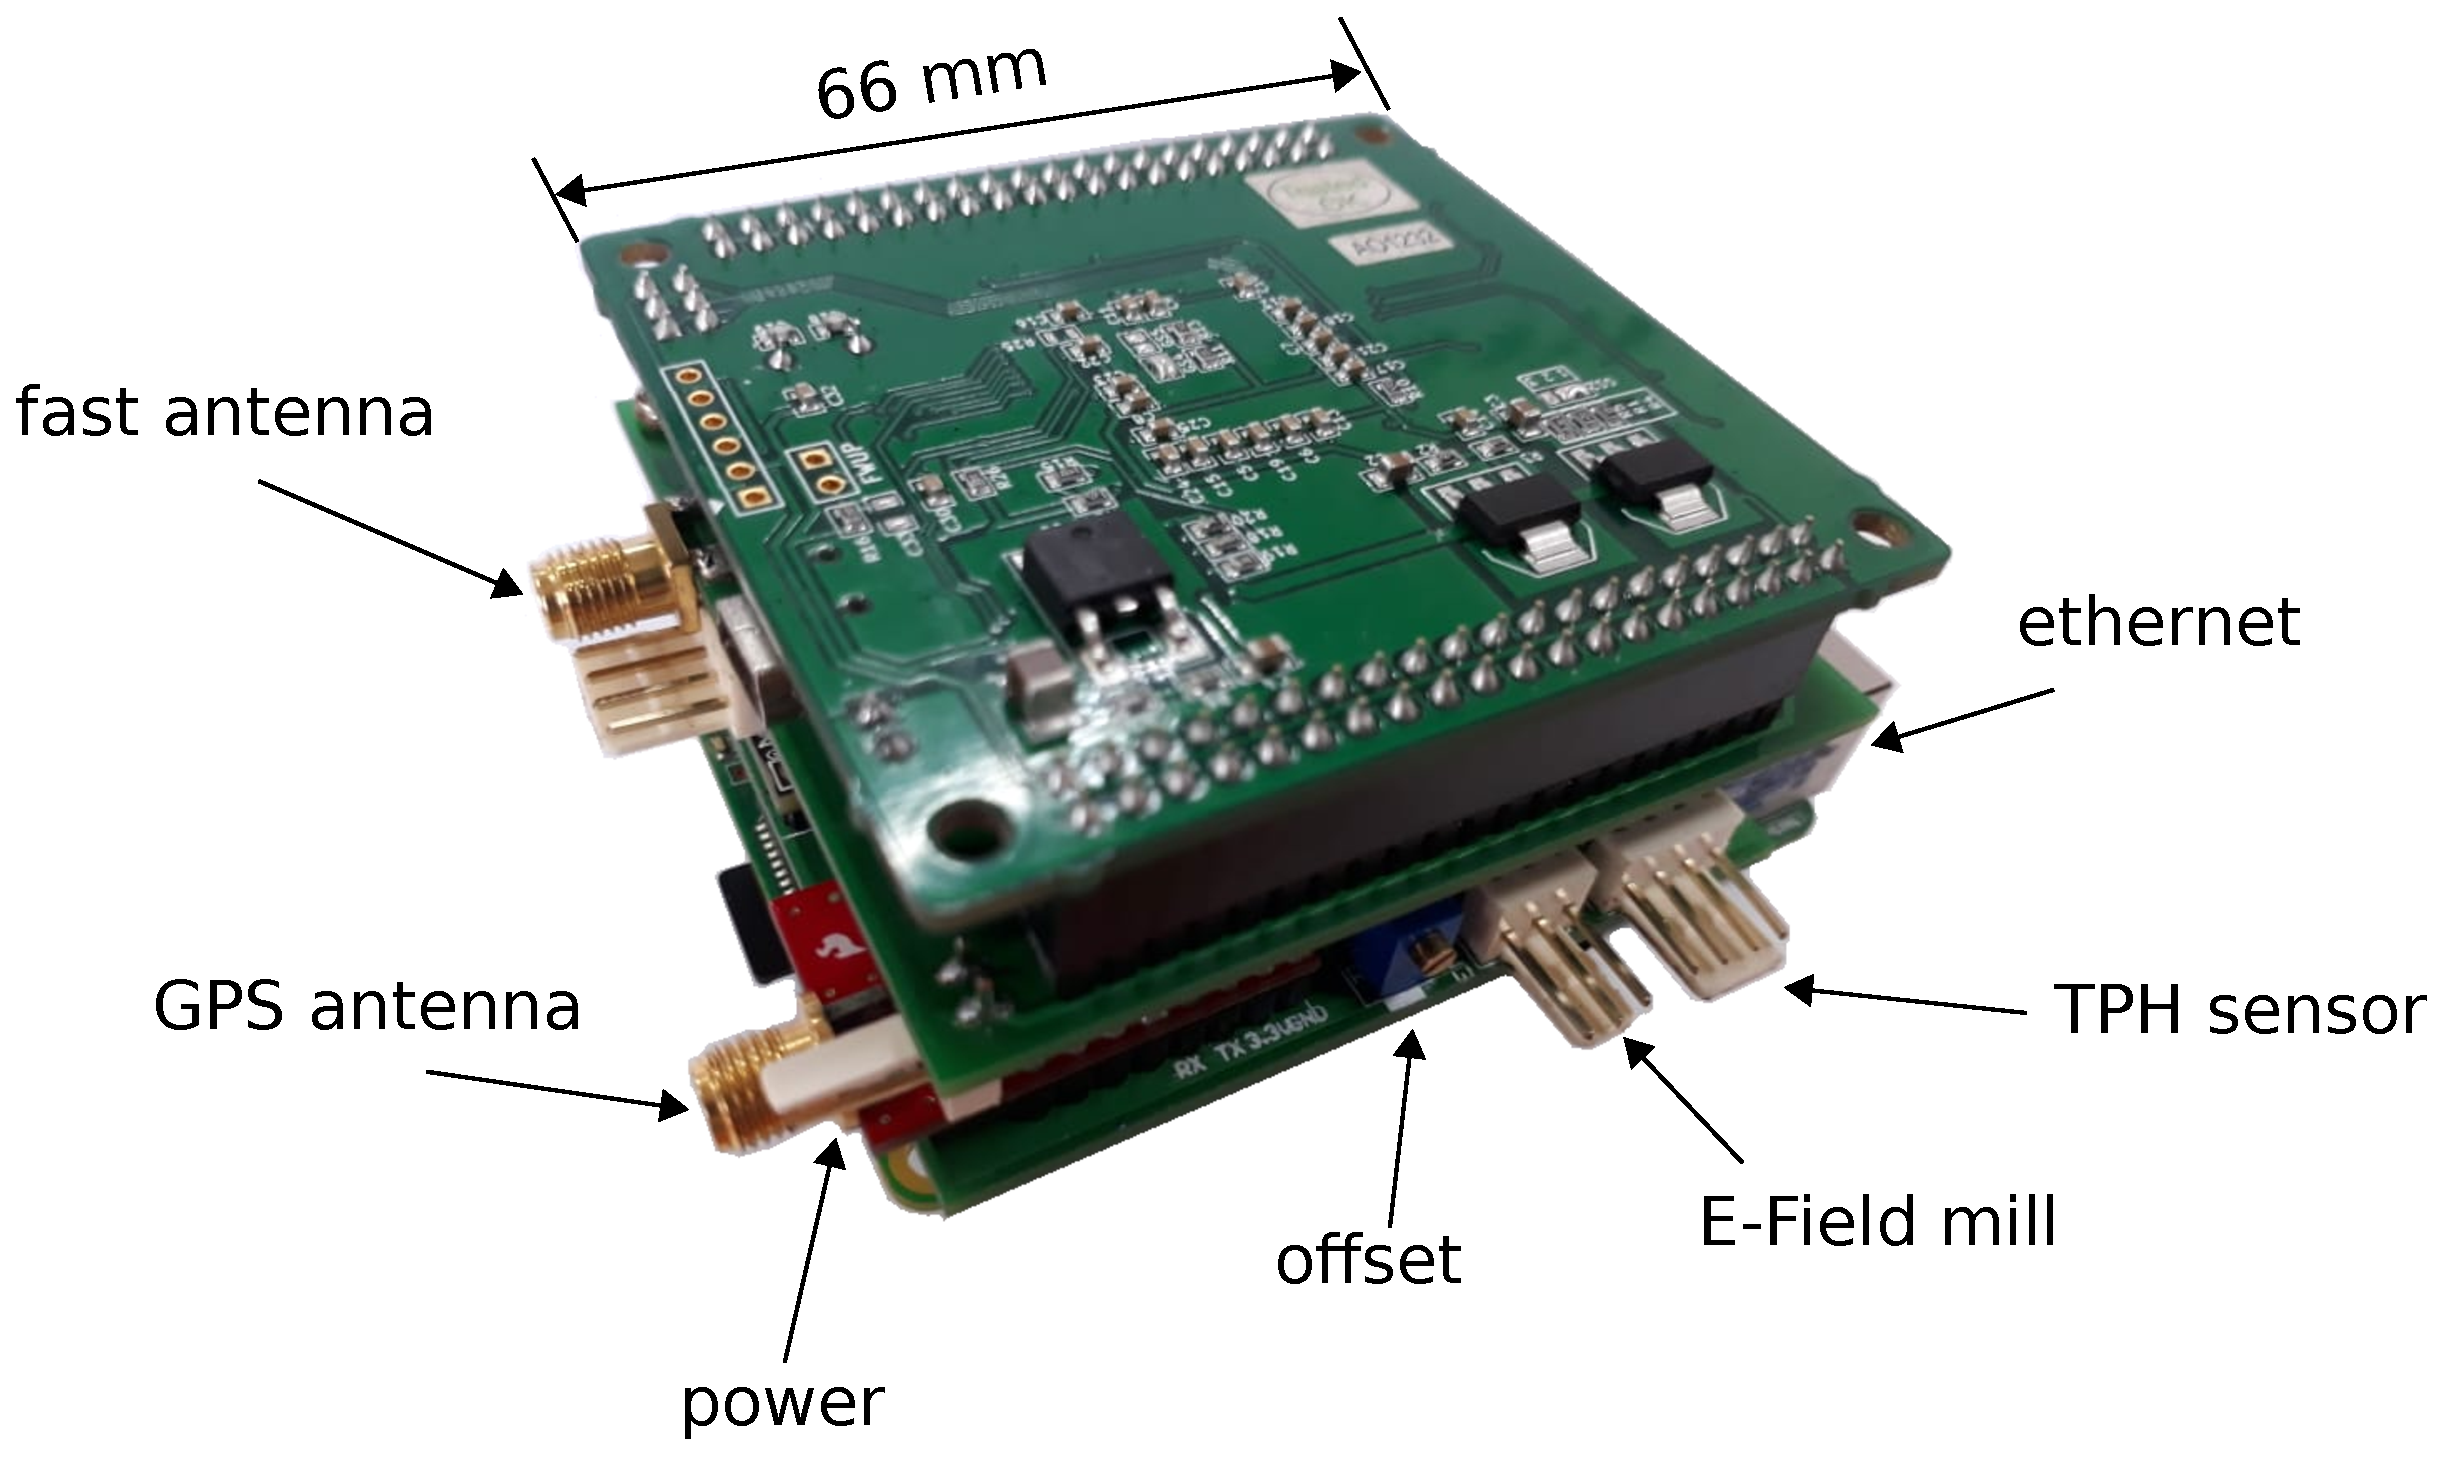
\includegraphics[width=0.55\textwidth]{Figures/Station.eps}
\caption{\label{station} The monitoring station hardware. The electronics frontend and readout for the fast and slow E-field components are mounted over the SCB Raspberry Pi as a shield. External connectors for powering, weather sensors, GPS antenna, fast antenna, E-field mill, and Ethernet communication are placed on the cube faces.}
\end{center}
\end{figure}

The monitoring station is operated by a Single Computer Board (SCB) Raspberry Pi running under Raspbian Wheezy. Apart from the E-field mill, other peripherals are connected in order to get information about the weather at the observation place. Temperature, relative humidity, and atmospheric pressure are measured using the BME280 sensor with an accuracy of $\pm$1 $^{\circ}$C, $\pm$3 $\%$RH, and $\pm$1 hPa respectively. A GPS Venus 638FLPx synchronizes temporally the data acquisition system with a spatial accuracy of 2.5 m and a time accuracy of 60 ns. The GPS data is received by the UART protocol at 9600 bps.

Additionally, a fast antenna detects lightning events that are digitized by a 12 bits fast ADC (AD9235) at 1 MSPS in an acquiring time window of 1 s. The digital signal is temporally stored in a 16 Mbit NOR Flash memory (SST39VF1601C) when the input pulse provided by a flat antenna exceeds the trigger threshold. This processing is performed by a Spartan 6 FPGA Development Board (Mimas). Once the acquisition window ends, the data is permanently stored in the SD card of the SCB with a timestamp of 10 ns resolution. The localization of the lightning strike point is estimated by using a trilateration algorithm \cite{MialdeaFlor2019}.

The monitoring station data can be acceded by an Ethernet link from a central server. A picture of the station hardware is displayed in figure \ref{station}.

\section{First measurements}

\begin{figure}[h]
\begin{center}
\includegraphics[width=0.48\textwidth]{Figures/Slow.eps}
\includegraphics[width=.48\textwidth]{Figures/Potential.eps}
\includegraphics[width=0.48\textwidth]{Figures/Temperatura.eps}
\includegraphics[width=.48\textwidth]{Figures/Humidity.eps}
\caption{\label{cal_fuente} Atmospheric variables recorded during the thunderstorm event 09-11-2019. A negative electric field (red-line) with a maximum of 15 kV/m was recorded after the storm-cloud formation $\sim$ 2 km above the observation place. The cloud-ground potential (black-line) was estimated using the electric field and the cloud base. The cloud base was modeled taking into account the measurements of temperature (blue-line) and relative humidity (green-line) as it is exposed by Lawrence et. al. \cite{Lawrence2005}.}
\label{cal_fuente}
\end{center}
\end{figure}

In this section, we show the results of the first measurements recorded during a thunderstorm event in 09-11-2019 at Bucaramanga, Colombia. The event lasts about 2 hours recording an electric field peak of -15 kV/m. The atmospheric electric field recovers the steady-state after at least half-hour of continuous lightning activity showing a ripple of 4 kV/m. The cloud-to-ground potential is proportional to the measured electric field and inverse to the cloud base distance. The storm cloud-base was estimated by using a model based on the relative humidity and temperature \cite{Lawrence2005} being close to 2 km. The atmospheric potential was $\sim$ 27 $\times$10$^6$ V at the electric field maximum.

A temperature drop of 3.5$^{\circ}$ was recorded at the event beginning, similarly, the relative humidity decreased from 88$\%$ to 76$\%$ due to the increment of the wind speed which dissipates the water molecules into the air. During the thunderstorm period, several lightning events occurred releasing a high amount of the charge stored inside the storm clouds. In figure \ref{light} we show 4 lightning events. 

\begin{figure}[h]
\begin{center}
\includegraphics[width=0.6\textwidth]{Figures/lightning.eps}
\caption{\label{light} Lightning events during the thunderstorm 09-11-2019. The arrows indicate the cloud-ground discharges along the storm period.}
\label{cal_fuente}
\end{center}
\end{figure}
 
The first event represents an electric field variation of near 8.5 kV/m in less than one minute. The estimation of the current flowing from the cloud to the ground is possible if the strike distance of the discharge is known. The charges accumulated in the storm cloud are released along the time ($\sim$ 10 min ) by lightning discharges until the electric field drops around the baseline.

\section{Conclusions}

Several studies have demonstrated a direct relationship between the atmospheric electric field and the flux of charged particles at ground level. However, the lack of enough data bout the electric field strength at cosmic rays observatories limits the understanding and analysis of such phenomena. In this work, we presented the design and first measurements of a monitoring station for measuring the slow and fast behavior of the atmospheric electric field fulfilling timing and triggering requirements needed to cross the recorded data with the counting rate measurements of particle detectors.
We show preliminary measurements where correlations between temperature, relative humidity, and thunderstorm development were found. The electric field of such thunderstorm episodes rose up to -15 kV/m with a cloud-ground potential of $\sim$ 27 $\times$10$^6$ V. Additionally, we identified some lightning events which caused an electric field variation of the order of 8.5 kV/m.

\section*{References}
\bibliographystyle{unsrt}
\bibliography{iopart-num.bib}

% \begin{thebibliography}{9}
% \bibitem{iopartnum} IOP Publishing is to grateful Mark A Caprio, Center for Theoretical Physics, Yale University, for permission to include the {\tt iopart-num} \BibTeX package (version 2.0, December 21, 2006) with  this documentation. Updates and new releases of {\tt iopart-num} can be found on \verb"www.ctan.org" (CTAN). 
% \end{thebibliography}

\end{document}


